\documentclass[border=3pt]{standalone}
\usepackage{fontspec}
\setmainfont{Times New Roman}
\usepackage{pgfplots}
\pgfplotsset{compat=1.18}
\usetikzlibrary{arrows.meta,calc,positioning,shapes.geometric}
\definecolor{forest}{HTML}{346E57}
\definecolor{sage}{HTML}{E8EFEA}
\definecolor{clay}{HTML}{B77E60}
\definecolor{gray}{HTML}{718078}
\definecolor{rule}{HTML}{B7C3BA}
\definecolor{ink}{HTML}{000000}
\begin{document}
\hyphenpenalty=10000\exhyphenpenalty=10000
\fontsize{10}{12}\selectfont
\renewcommand{\small}{\fontsize{9}{11}\selectfont}
\renewcommand{\scriptsize}{\fontsize{8}{10}\selectfont}
\resizebox{16cm}{!}{%
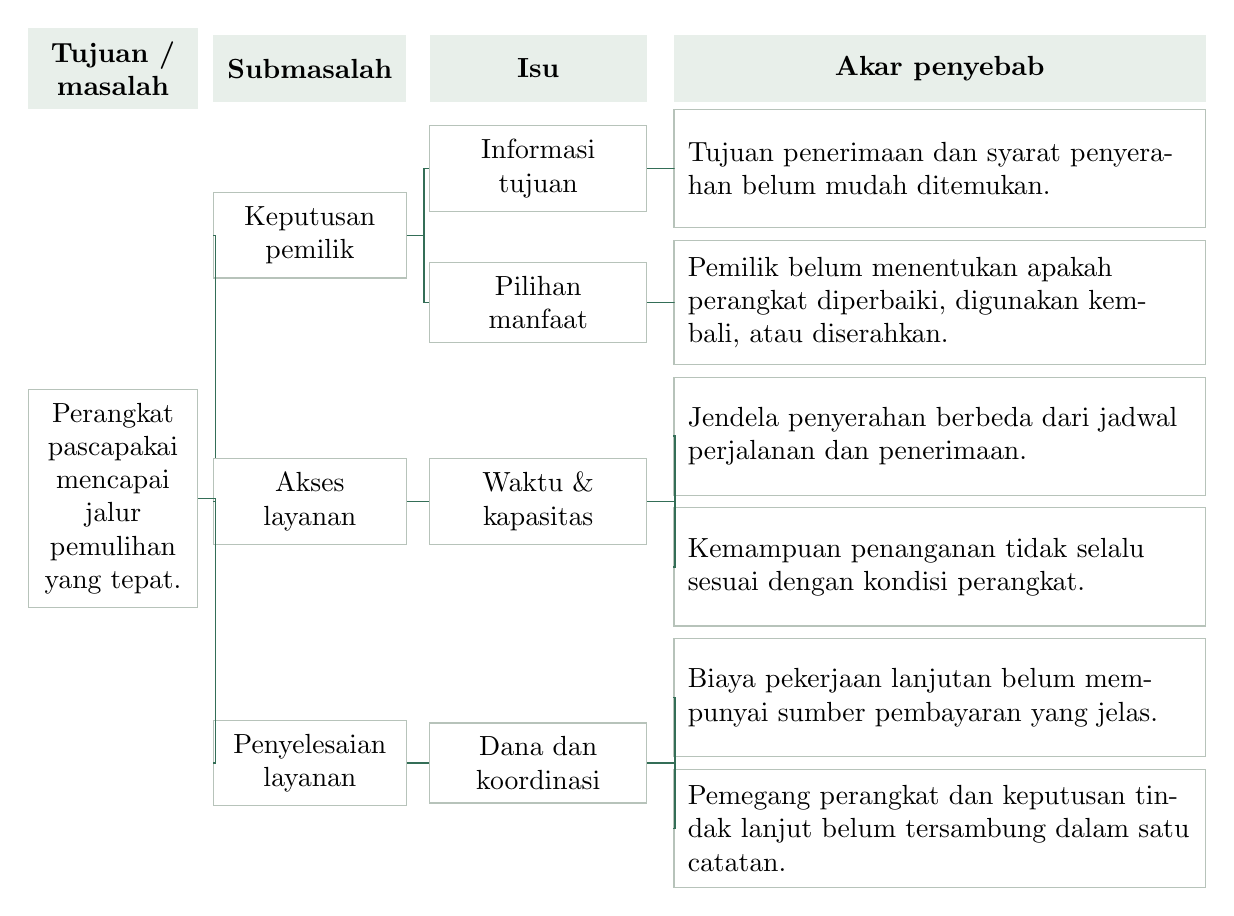
\begin{tikzpicture}[x=1cm,y=1cm,box/.style={draw=rule,line width=.45pt,fill=white,align=center,inner sep=5pt},edge/.style={draw=forest,line width=.6pt}]
\node[fill=sage,text width=1.8cm,minimum height=.85cm,align=center,inner sep=5pt,font=\bfseries] at (1.0,.52) {Tujuan / masalah};
\node[fill=sage,text width=2.1cm,minimum height=.85cm,align=center,inner sep=5pt,font=\bfseries] at (3.5,.52) {Submasalah};
\node[fill=sage,text width=2.4cm,minimum height=.85cm,align=center,inner sep=5pt,font=\bfseries] at (6.4,.52) {Isu};
\node[fill=sage,text width=6.4cm,minimum height=.85cm,align=center,inner sep=5pt,font=\bfseries] at (11.5,.52) {Akar penyebab};
\node[box,text width=1.8cm] (goal) at (1,-4.9399999999999995) {Perangkat pascapakai mencapai jalur pemulihan yang tepat.};
\node[box,text width=2.1cm] (b0) at (3.5,-1.6) {Keputusan pemilik};
\draw[edge] (goal.east) -- ++(.22,0) |- (b0.west);
\node[box,text width=2.1cm] (b1) at (3.5,-4.98) {Akses layanan};
\draw[edge] (goal.east) -- ++(.22,0) |- (b1.west);
\node[box,text width=2.1cm] (b2) at (3.5,-8.299999999999999) {Penyelesaian layanan};
\draw[edge] (goal.east) -- ++(.22,0) |- (b2.west);
\node[box,text width=2.4cm] (i0x0) at (6.4,-0.75) {Informasi tujuan};
\draw[edge] (b0.east) -- ++(.22,0) |- (i0x0.west);
\node[box,text width=2.4cm] (i0x1) at (6.4,-2.45) {Pilihan manfaat};
\draw[edge] (b0.east) -- ++(.22,0) |- (i0x1.west);
\node[box,text width=2.4cm] (i1x0) at (6.4,-4.98) {Waktu \& kapasitas};
\draw[edge] (b1.east) -- ++(.22,0) |- (i1x0.west);
\node[box,text width=2.4cm] (i2x0) at (6.4,-8.299999999999999) {Dana dan koordinasi};
\draw[edge] (b2.east) -- ++(.22,0) |- (i2x0.west);
\node[box,text width=6.4cm,align=left,minimum height=1.5cm] (c0) at (11.5,-0.75) {Tujuan penerimaan dan syarat penyerahan belum mudah ditemukan.};
\draw[edge] (i0x0.east) -- ++(.35,0) |- (c0.west);
\node[box,text width=6.4cm,align=left,minimum height=1.58cm] (c1) at (11.5,-2.45) {Pemilik belum menentukan apakah perangkat diperbaiki, digunakan kembali, atau diserahkan.};
\draw[edge] (i0x1.east) -- ++(.35,0) |- (c1.west);
\node[box,text width=6.4cm,align=left,minimum height=1.5cm] (c2) at (11.5,-4.15) {Jendela penyerahan berbeda dari jadwal perjalanan dan penerimaan.};
\draw[edge] (i1x0.east) -- ++(.35,0) |- (c2.west);
\node[box,text width=6.4cm,align=left,minimum height=1.5cm] (c3) at (11.5,-5.81) {Kemampuan penanganan tidak selalu sesuai dengan kondisi perangkat.};
\draw[edge] (i1x0.east) -- ++(.35,0) |- (c3.west);
\node[box,text width=6.4cm,align=left,minimum height=1.5cm] (c4) at (11.5,-7.47) {Biaya pekerjaan lanjutan belum mempunyai sumber pembayaran yang jelas.};
\draw[edge] (i2x0.east) -- ++(.35,0) |- (c4.west);
\node[box,text width=6.4cm,align=left,minimum height=1.5cm] (c5) at (11.5,-9.129999999999999) {Pemegang perangkat dan keputusan tindak lanjut belum tersambung dalam satu catatan.};
\draw[edge] (i2x0.east) -- ++(.35,0) |- (c5.west);
\end{tikzpicture}
}

\end{document}
